\chapter{Zig Zag Puzzler}
For the Zig Zag puzzler, there are 2 playing modes. Therefore,each mode will correspond to one model. The significant difference between them are the three-dimensional system of coordinate.
Above all, I would like to define all the variables based on the piece.
\section{playing mode 1 - CSP model}
\label{sec:CSP model1}
Firstly, I'd like to explain how to calculate the position based on the board.
\begin{center}
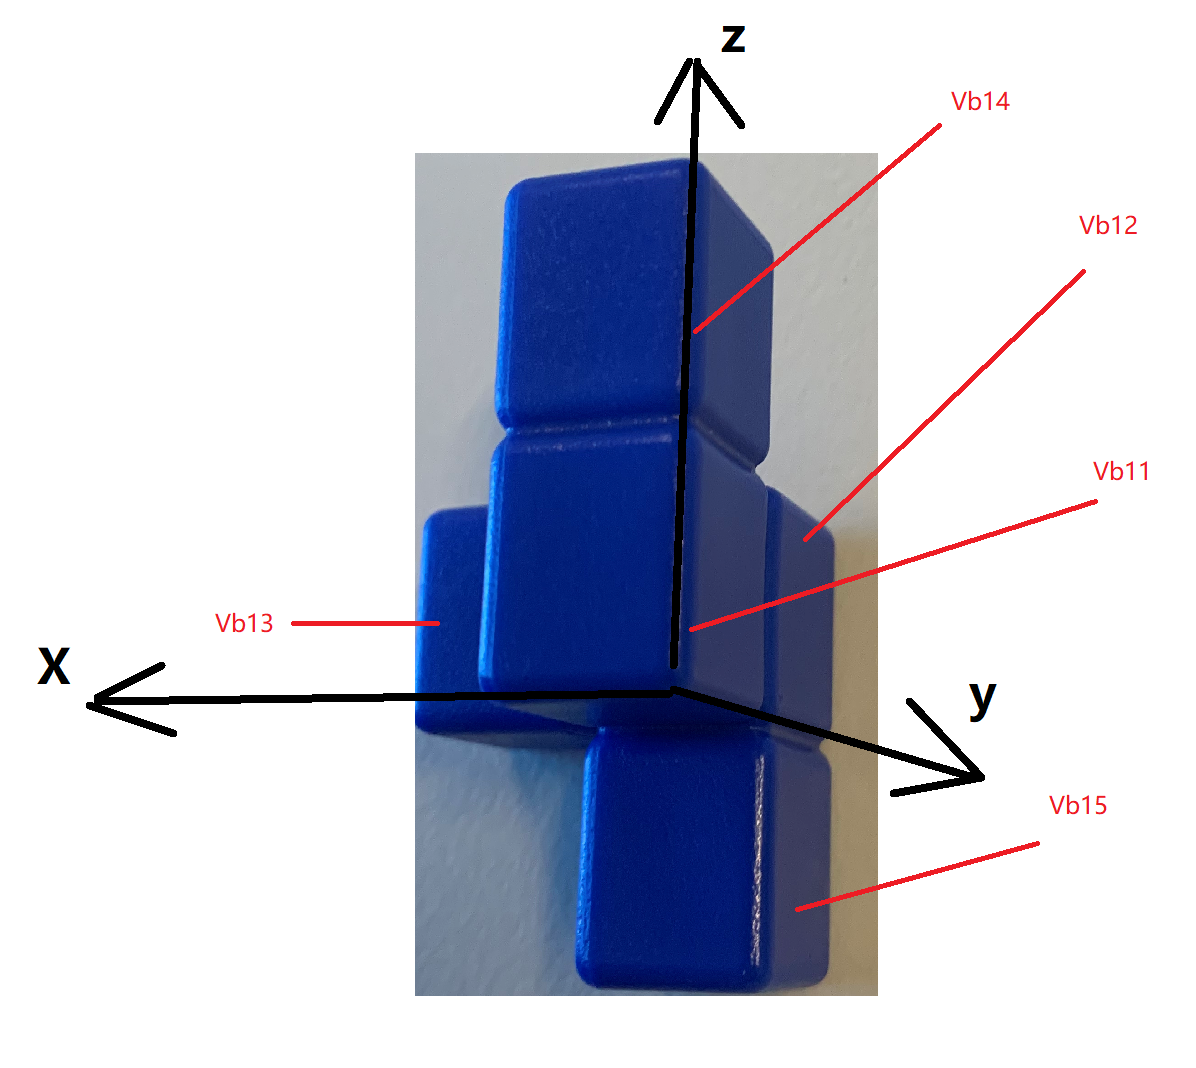
\includegraphics[scale=0.5]{game2blue1.png}\\
the variable explanation of blue1\\
\end{center}
\begin{center}
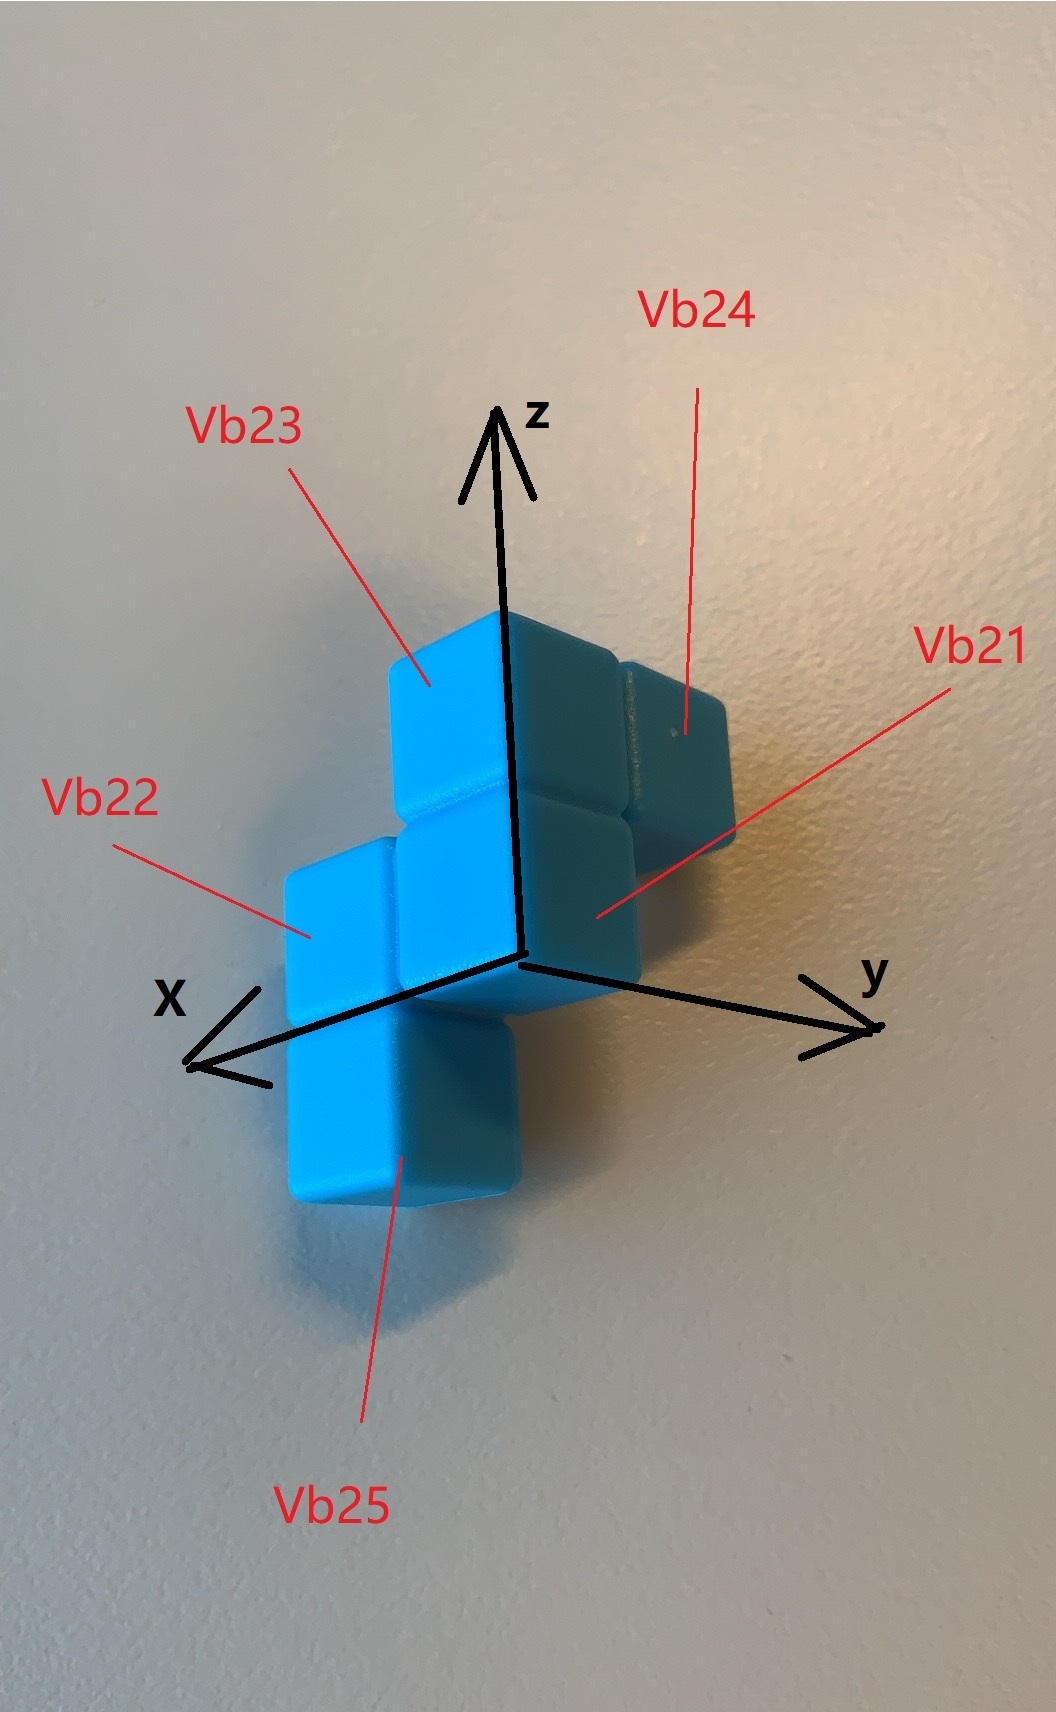
\includegraphics[scale=0.5]{game2blue2.jpg}\\
the variable explanation of blue2
\end{center}
\begin{center}
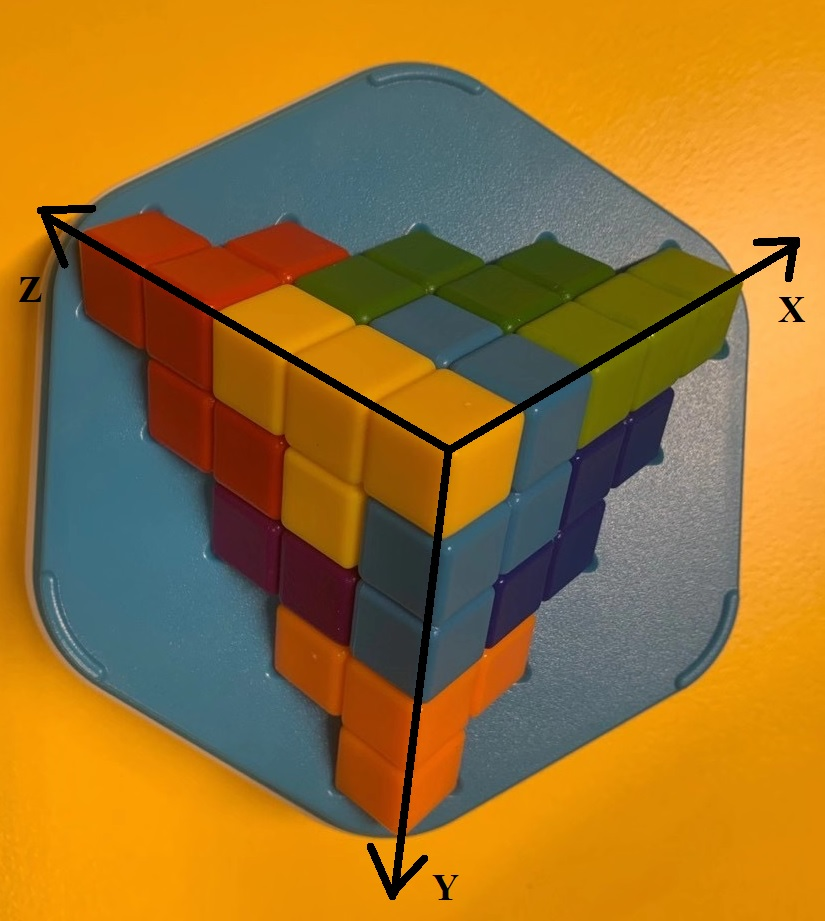
\includegraphics[scale=0.5]{ZIGZAGmodel1board.jpg} \\
explanation of zig zag puzzler model1
\end{center}
\subsection{Variables}
\begin{align*}
\VUnits=\{&V_{y1},V_{y2},V_{y3},V_{y4},\\&V_{b11},V_{b12},V_{b13},V_{b14},
V_{b15},\\&V_{b21},V_{b22},V_{b23},V_{b24},V_{b25},\\&V_{g11},V_{g12},V_{g13},V_{g14},\\&V_{g21},V_{g22},V_{g23},\\&V_{r11},
V_{r12},V_{r13},\\&V_{r21},V_{r22},V_{r23},\\&V_{o1},V_{o2},V_{o3},V_{o4},\\&V_{p1},V_{p2},V_{p3},V_{p4}\}
\end{align*}
\subsection{Domains}
\begin{align*}
For \hspace{1ex} all \hspace{1ex} v \in \VUnits \hspace{1ex},\hspace{1ex} D(v)=\{&(i,j,k) \in \mathbb{Z} \times \mathbb{Z}	\times \mathbb{Z} \mid  0<i \leq 5 \hspace{1ex} , \hspace{1ex} 0<j \leq 5,\hspace{1ex} 0<k \leq 5,\\& i+j\leq 6,\hspace{1ex} j+k\leq 6,\hspace{1ex}i+k\leq 6,\hspace{1ex}i+j+k\leq 7\}
\end{align*}
\subsection{Constraints}
\begin{small}
\begin{align*}
&\Cons{b11}{b12}{b13}{b14}{b15}=\{\\
&((a,b,c),(d,e,f),(g,h,i),(j,k,l),(m,n,o))\in \Domain {b11} \times \Domain{b12}\times \Domain{b13}\times \Domain{b14}\times \Domain{b15} \mid\\
&(d=a , e=b+1,f=c , g=a+1,h=b+1,i=c ,j=a ,k=b ,l=c+1,m=a ,n=b+1,o=c-1)or\\
&(d=a-1,e=b , f=c,g=a-1,h=b+1,i=c ,j=a ,k=b ,l=c+1,m=a-1,n=b ,o=c-1)or\\
&(d=a , e=b-1,f=c , g=a-1,h=b-1,i=c ,j=a ,k=b ,l=c+1,m=a ,n=b-1,o=c-1)or\\
&(d=a+1,e=b , f=c , g=a+1,h=b-1,i=c ,j=a ,k=b ,l=c+1,m=a+1,n=b ,o=c-1)or\\
&(d=a , e=b-1, f=c , g=a+1,h=b-1,i=c ,j=a ,k=b ,l=c-1,m=a ,n=b-1,o=c+1)or\\
&(d=a+1,e=b , f=c , g=a+1,h=b+1,i=c ,j=a ,k=b ,l=c-1,m=a+1,n=b ,o=c+1)or\\
&(d=a , e=b+1, f=c , g=a-1,h=b+1,i=c ,j=a ,  k=b ,l=c-1,m=a ,n=b+1,o=c+1)or\\
&(d=a-1,e=b ,f=c , g=a-1,h=b-1,i=c ,j=a ,k=b ,l=c-1,m=a-1,n=b ,o=c+1)or\\
&(d=a ,e=b ,f=c+1, g=a+1,h=b ,i=c+1 ,j=a ,k=b-1,l=c ,m=a ,n=b+1,o=c+1)or\\
&(d=a ,e=b-1,f=c , g=a+1,h=b-1,i=c  ,j=a ,k=b ,l=c-1,m=a ,n=b-1,o=c+1)or\\
&(d=a ,e=b ,f=c-1, g=a+1,h=b ,i=c-1 ,j=a ,k=b+1,l=c ,m=a ,n=b-1,o=c-1)or\\
&(d=a ,e=b+1,f=c , g=a-1,h=b+1,i=c  ,j=a ,k=b ,l=c-1,m=a ,n=b+1,o=c+1)or\\
&(d=a ,e=b ,f=c+1, g=a-1,h=b ,i=c+1 ,j=a ,k=b+1,l=c ,m=a ,n=b-1,o=c+1)or\\
&(d=a ,e=b-1,f=c , g=a-1,h=b-1,i=c  ,j=a ,k=b ,l=c+1,m=a ,n=b-1,o=c-1)or\\
&(d=a ,e=b ,f=c-1, g=a-1,h=b ,i=c-1 ,j=a ,k=b-1,l=c ,m=a ,n=b+1,o=c-1)or\\
&(d=a ,e=b+1,f=c , g=a ,h=b+1,i=c+1 ,j=a-1,k=b ,l=c ,m=a+1,n=b+1,o=c )or\\
&(d=a ,e=b ,f=c+1, g=a ,h=b-1,i=c+1 ,j=a-1,k=b ,l=c ,m=a+1,n=b ,o=c+1)or\\
&(d=a ,e=b-1,f=c , g=a ,h=b-1,i=c-1 ,j=a-1,k=b ,l=c ,m=a+1,n=b-1,o=c )or\\
&(d=a ,e=b+1,f=c , g=a-1,h=b+1,i=c  ,j=a ,k=b ,l=c-1,m=a ,n=b+1,o=c+1)or\\
&(d=a ,e=b ,f=c+1, g=a-1,h=b ,i=c+1 ,j=a ,k=b+1,l=c ,m=a ,n=b-1,o=c+1)or\\
&(d=a ,e=b-1,f=c , g=a-1,h=b-1,i=c  ,j=a ,k=b ,l=c+1,m=a ,n=b-1,o=c-1)or\\
&(d=a ,e=b ,f=c-1, g=a-1,h=b ,i=c-1,j=a ,k=b-1,l=c ,m=a ,n=b+1,o=c-1)\}
\end{align*}
\end{small}
\begin{small}
\begin{align*}
&\Cons{b21}{b22}{b23}{b24}{b25}=\{
\\&((a,b,c),(d,e,f),(g,h,i),(j,k,l),(m,n,o))\in \Domain {b21} \times \Domain{b22}\times \Domain{b23}\times \Domain{b24}\times \Domain{b25} \mid
\\&(d=a+1,e=b ,f=c , g=a ,h=b ,i=c+1,j=a ,k=b+1,l=c+1,m=a+1,n=b ,o=c-1)or
\\&(d=a ,e=b+1,f=c , g=a ,h=b ,i=c+1,j=a-1,k=b ,l=c+1,m=a ,n=b+1,o=c-1)or
\\&(d=a-1,e=b ,f=c , g=a ,h=b ,i=c+1,j=a ,k=b-1,l=c+1,m=a-1,n=b ,o=c-1)or
\\&(d=a ,e=b-1,f=c , g=a ,h=b ,i=c+1,j=a+1,k=b ,l=c+1,m=a ,n=b-1,o=c-1)or
\\&(d=a+1,e=b ,f=c , g=a ,h=b ,i=c-1,j=a ,k=b-1,l=c-1,m=a+1,n=b ,o=c+1)or
\\&(d=a ,e=b+1,f=c , g=a ,h=b ,i=c-1,j=a+1,k=b ,l=c-1,m=a ,n=b+1,o=c+1)or
\\&(d=a-1,e=b ,f=c , g=a ,h=b ,i=c-1,j=a ,k=b+1,l=c-1,m=a-1,n=b ,o=c+1)or
\\&(d=a ,e=b-1,f=c , g=a ,h=b ,i=c-1,j=a-1,k=b ,l=c-1,m=a ,n=b-1,o=c+1)or
\\&(d=a+1,e=b ,f=c , g=a ,h=b-1,i=c ,j=a ,k=b-1,l=c+1,m=a+1,n=b+1,o=c )or
\\&(d=a+1,e=b ,f=c , g=a ,h=b ,i=c-1,j=a ,k=b-1,l=c-1,m=a+1,n=b ,o=c+1)or
\\&(d=a+1,e=b ,f=c , g=a ,h=b+1,i=c ,j=a ,k=b+1,l=c-1,m=a+1,n=b-1,o=c )or
\\&(d=a-1,e=b ,f=c , g=a ,h=b ,i=c-1,j=a ,k=b+1,l=c-1,m=a-1,n=b ,o=c+1)or
\\&(d=a-1,e=b ,f=c , g=a ,h=b+1,i=c ,j=a ,k=b+1,l=c+1,m=a-1,n=b-1,o=c )or
\\&(d=a-1,e=b ,f=c , g=a ,h=b ,i=c+1,j=a ,k=b-1,l=c+1,m=a-1,n=b ,o=c-1)or
\\&(d=a-1,e=b ,f=c , g=a ,h=b-1,i=c ,j=a ,k=b-1,l=c-1,m=a-1,n=b+1,o=c )or
\\&(d=a ,e=b ,f=c+1, g=a-1,h=b ,i=c ,j=a-1,k=b+1,l=c ,m=a+1,n=b ,o=c+1)or
\\&(d=a ,e=b-1,f=c , g=a-1,h=b ,i=c ,j=a-1,k=b ,l=c+1,m=a+1,n=b-1,o=c )or
\\&(d=a ,e=b ,f=c-1, g=a-1,h=b ,i=c ,j=a-1,k=b-1,l=c ,m=a+1,n=b ,o=c-1)or
\\&(d=a-1,e=b ,f=c , g=a ,h=b ,i=c-1,j=a ,k=b+1,l=c-1,m=a-1,n=b ,o=c+1)or
\\&(d=a-1,e=b ,f=c , g=a ,h=b+1,i=c ,j=a ,k=b+1,l=c+1,m=a-1,n=b-1,o=c )or
\\&(d=a-1,e=b ,f=c , g=a ,h=b ,i=c+1,j=a ,k=b-1,l=c+1,m=a-1,n=b ,o=c-1)or
\\&(d=a-1,e=b ,f=c , g=a ,h=b-1,i=c ,j=a ,k=b-1,l=c-1,m=a-1,n=b+1,o=c )\}
\end{align*}
\end{small}
\section{playing mode 2 - CSP model}
\begin{center}
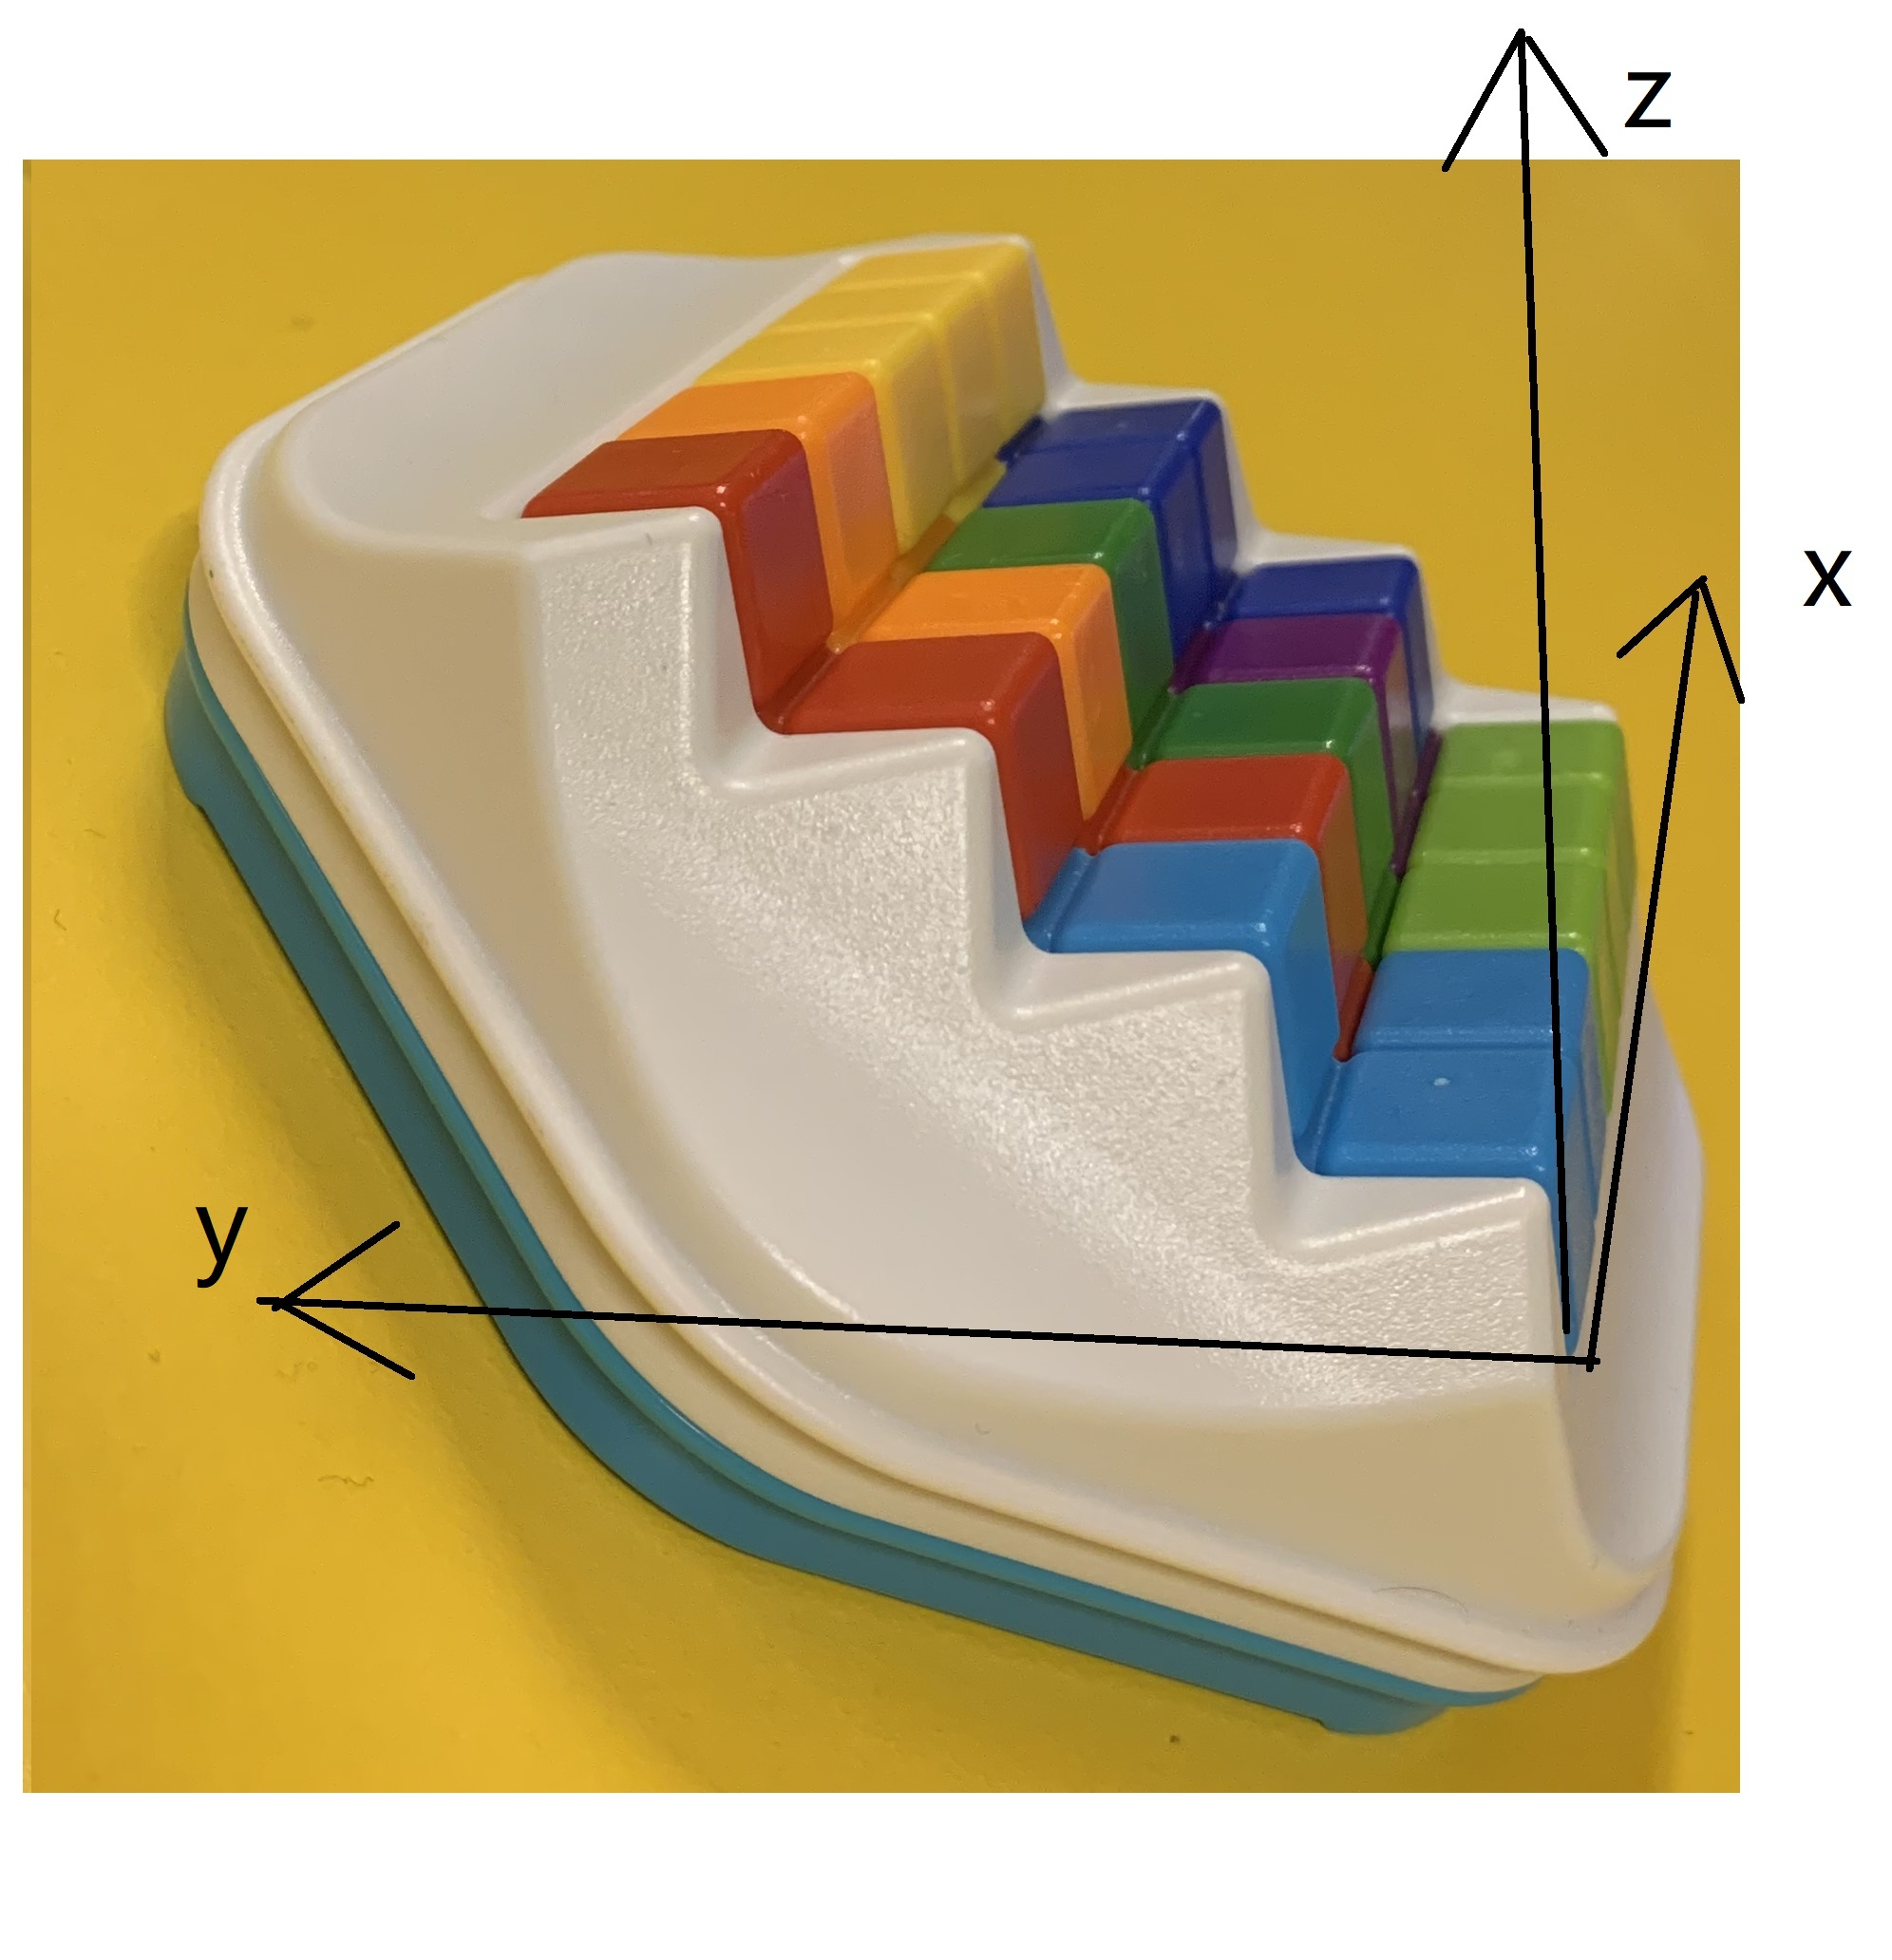
\includegraphics[scale=0.2]{ZIGZAGmodel2board.jpg} \\
explanation of zig zag puzzler model2
\end{center}
\label{sec:CSP model2}
\subsection{Variables}
\begin{align*}
\VUnits=\{&V_{y1},V_{y2},V_{y3},V_{y4},\\&V_{b11},V_{b12},V_{b13},V_{b14},
V_{b15},\\&V_{b21},V_{b22},V_{b23},V_{b24},V_{b25},\\&V_{g11},V_{g12},V_{g13},V_{g14},\\&V_{g21},V_{g22},V_{g23},\\&V_{r11},
V_{r12},V_{r13},\\&V_{r21},V_{r22},V_{r23},\\&V_{o1},V_{o2},V_{o3},V_{o4},\\&V_{p1},V_{p2},V_{p3},V_{p4}\}
\end{align*}
\subsection{Domains}
\begin{align*}
For \hspace{1ex} all \hspace{1ex} v \in \VUnits \hspace{1ex},\hspace{1ex} D(v)=\{&(i,j,k) \in \mathbb{Z} \times \mathbb{Z}	\times \mathbb{Z} \mid  0<i \leq 5 \hspace{1ex} , \hspace{1ex} 0<j \leq 4,\hspace{1ex} 0<k \leq 4,j=k\} \hspace{1ex}\cup\\
\{&(i,j,k) \in \mathbb{Z} \times \mathbb{Z}	\times \mathbb{Z} \mid  0<i \leq 5 \hspace{1ex} , \hspace{1ex} 0<j \leq 4,\hspace{1ex} 0<k \leq 3,j=k+1\}
\end{align*}